\documentclass{beamer}

\usepackage[utf8]{inputenc}
\usepackage[T1]{fontenc}

\usepackage[english]{babel}
\usepackage{amsmath}
\usepackage{cleveref}
\usepackage{amssymb}
\usepackage{mathtools}

%%Numbers, expectation
\newcommand{\N}{\mathbb{N}}
\newcommand{\E}{\mathbb{E}}
\renewcommand{\P}{\mathbb{P}}
\newcommand{\Var}{\mathbb{V}}
\newcommand{\R}{\mathbb{R}}
\newcommand{\D}{\mathcal{D}}
\newcommand{\B}{\mathcal{B}}
\newcommand{\Dh}{\D_h}
\renewcommand{\phi}{\varphi}
\newcommand*\diff{\mathop{}\!\mathrm{d}} % integral

%% mathoperator
\DeclareMathOperator*{\argmax}{arg\,max}
\DeclareMathOperator*{\argmin}{arg\,min}
\DeclareMathOperator*{\dom}{dom}
\DeclareMathOperator*{\sign}{sign}
\DeclareMathOperator*{\diag}{diag}

\DeclareMathOperator*{\Cov}{Cov}
\DeclareMathOperator*{\Cor}{Corr}
\DeclareMathOperator*{\Id}{Id}

%proximal operator
\newcommand{\prox}[3][]{\operatorname{prox}^{#1}_{#2}\left(#3 \right)}

\usepackage{xcolor}

%% sort citations by increasing number
\usepackage[sort,nocompress]{cite}

\usepackage{graphicx}% http://ctan.org/pkg/graphicx
\graphicspath{{../figures/}{../../figures}{../../memes}} %Setting the graphicspath
\usepackage{caption,subcaption}

\usepackage{tikz}
\usepackage{pgfplots}
\usetikzlibrary{backgrounds}
\usetikzlibrary{intersections}
\usepgfplotslibrary{fillbetween}

% \usepackage[right]{showlabels}


%%
\theoremstyle{plain}
\newtheorem{prop}{Proposition}[section]
\newtheorem{algo}{Algorithm}[section]
\newtheorem{assumption}{Assumption}
\theoremstyle{remark}
\newtheorem{remark}{Remark}[section]

% cref
\crefname{assumption}{Assumption}{Assumptions}
\crefname{equation}{}{}

\usepackage{autonum}

\usepackage{bm} %% bold math symbols

\usepackage{bbm} %% for \mathbbm{1}


% algorithmic environment
\usepackage{algorithm}
\usepackage[noend]{algpseudocode}

% for some reason this was required on one void linux installation (but not the other)
\usepackage{sansmathaccent}
\pdfmapfile{+sansmathaccent.map}

\author{Axel Böhm}

% shows which section we're in
\usetheme{Darmstadt}

% page number
\setbeamertemplate{footline}[frame number]
\setbeamercolor{page number in head/foot}{fg=gray}


% display things like onslide or visible already before but grayed out
\setbeamercovered{transparent}

% set the itemize item symbol as a diamond
\setbeamertemplate{itemize item}{$\diamond$}
% set the itemize subitem symbol as a triangle
\setbeamertemplate{itemize subitem}{$\blacktriangleright$}

% set the enumerate item symbol as a roman numbers
\setbeamertemplate{enumerate item}{(\roman{enumi})}


% reference: https://yuxinchen2020.github.io/ele522_optimization/lectures/variance_reduction.pdf

\title{Variance reduction for stochastic gradient methods}
\date{\today}

\begin{document}
\maketitle
\frame{\tableofcontents[currentsection]}


\section{Introduction}%

\begin{frame}
  \frametitle{The finite sum probem}
  A common Task in (supervised) machine learning:
  \begin{equation}
    \min_{x\in \R^d} f(x) := \frac{1}{n} \sum_{i=1}^{n} \underbrace{f_i(x)}_{\textcolor{blue}{\text{loss for $i$-th sample}}} + \underbrace{\psi(x)}_{\textcolor{blue}{\text{regularizer}}}
  \end{equation}
  where the $i$-th sample is $(a_i, y_i)$.

  \textbf{Examples:}
  \begin{itemize}
    \item linear regression: $f_i(x) = {(a_i^T x -y_i)}^2$, and $\psi=0$
    \item logistic regression: $f_i(x) = \log(1+e^{-y_i a_i^T x})$, and $\psi=0$
          ``sigmoid function'' and logistic loss.
    \item Lasso: $f_i$ as for linear regression but $\psi(x) = \Vert x \Vert_i$
    \item SVM: $f_i(x) = \max \{0 , 1 - y_i a_i^T x\}$ and $\psi(x)= \Vert x \Vert^2$
  \end{itemize}
\end{frame}

\begin{frame}
  \frametitle{Gradient descent}
  \begin{algorithm}[H]
    \caption{(batch) GD}
    \begin{algorithmic}[1]
      \For{$k = 1,2, \dots$}
      \State{ $x_{k+1} = x_k  - \alpha_k \nabla f(x_k) $}
      \EndFor{}
    \end{algorithmic}
  \end{algorithm}

  \begin{itemize}
    \item gradient can be computed via
          \begin{equation}
            \nabla f(x) = \nabla \left(\sum_{i=1}^{n}f_i(x)\right) = \sum_{i=1}^{n} \nabla f_i(x_k)
          \end{equation}
    \item good convergence properties
    \item can be \textbf{expensive} if $n$ is large!
  \end{itemize}
\end{frame}


\begin{frame}
  \frametitle{Stochastic gradient descent}
  \begin{algorithm}[H]
    \caption{SGD}\label{sgd}
    \begin{algorithmic}[1]
      \For{$k = 1,2, \dots$}
      \State{pick $i_k$ uniform at random in $[n]$}
      \State{$x_{k+1} = x_k  - \alpha_k \nabla f_{i_k}(x_k)$}
      \EndFor{}
    \end{algorithmic}
  \end{algorithm}

  We already noticed that:
  \begin{itemize}
    \item unbiased: $\E[\nabla f_{i_k}(x)] = \sum_{i=1}^{n} \P[i=i_k] \nabla f_i(x) = \sum_{i=1}^{n} \frac{1}{n} \nabla f_i(x)$
    \item large stepsizes fail to suppress variability in the stoch.\ gradients $\rightarrow$ leads to oscillations
    \item decreasing stepsizes mitigate this problem but \textbf{slows down} convergence (too \emph{conservative})
  \end{itemize}

\end{frame}


\begin{frame}
  \frametitle{Recall SGD (template)}
  \begin{equation}
    x_{k+1} = x_k - \alpha_k g_k
  \end{equation}
  \begin{itemize}
    \item $g_k$ is an unbiased estimator of the true gradient $\nabla F(x_k)$
    \item convergence depends on \textbf{variance} $\E [ \Vert g_k - \nabla F(x_k) \Vert ] \le \sigma_g$
          (not strictly necessary)
    \item vanilla SGD uses $g_k = \nabla f_{i_k}(x_k)$ \\
          \textbf{issue:} $\sigma_g$ is non-negligible even close to the solution
    \item \textbf{Q:} can we choose $g_k$ in a different way to reduce variability?
  \end{itemize}

\end{frame}

\begin{frame}
  \frametitle{Minibatching}
  \begin{algorithm}[H]
    \caption{minibatch SGD}
    \begin{algorithmic}[1]
      \For{$k = 1,2, \dots$}
      \State{pick $I_k$ random subset of $[n]$ with $\vert I_k \vert = b $}
      \State{$x_{k+1} = x_k  - \alpha_k \sum_{i \in I_k} \nabla f_{i}(x_k)$}
      \EndFor{}
    \end{algorithmic}
  \end{algorithm}
  \begin{itemize}
    \item typically we make a (uniform) \emph{random} choice $i_k \in [n] = \{1, \dots, n\}$\\
          (or random reshuffling)
    \item by increasing the size to a \textbf{random subset} $I_k \subset [n]$ of size $b \ll n$ we can
          \begin{itemize}
            \item decrease variance
            \item increase cost only moderately,
            \item but cannot improve theoretical guarantees
          \end{itemize}
  \end{itemize}

\end{frame}


\begin{frame}
  \frametitle{A simple idea}
  Consider
  \begin{itemize}
    \item estimator $X$ for parameter $\mu$ ($\E[X]=\mu$ and $\Var[X]=\sigma^2$)
    \item want to keep unbiased but reduce variance
    \item find $Y$ such that $\E[Y] = 0$ but $\Cov (X,Y)$ is large and $\tilde{X}=X-Y$
    \item remains unbiased

          \begin{equation}
            \Var[\tilde{X}] = \Var[X]+\Var[Y]-2\Cov[X,Y]
          \end{equation}
    \item can be much smaller than $\V[X]$ if $X,Y$ are highly correlated
  \end{itemize}
\end{frame}

\section{SAG}%
\label{sec:}

\begin{frame}
  \frametitle{Stochastic average gradient (SAG), 2013}
  \begin{itemize}
    \item maintain table containing gradients $g_i$ of $f_i$
    \item at step $k = 1,2, \dots$ pick random $i_k \in [n]$ and
          \begin{equation}
            g_i^k := \nabla f_{i_k}(x^{k})
          \end{equation}
          set $g_{i}^k = g_i^{k-1}$ for all $i\neq i_k$ (remain the same)
    \item Update
          \begin{equation}
            x^{k+1} = x^k - \alpha_k \frac{1}{n} \sum_{i=1}^{n} g_i^k
          \end{equation}
    \item assuming gradients do not change too much along trajectory
    \item gradient estimator \textcolor{red}{no longer unbiased}
    \item Isn't it expensive to average these gradients?
          \begin{equation}
            x^{k+1} = x^k -u \alpha_k  \Big( \frac{g_{i_k}^k}{n} - \frac{g_{i_k}^{k-1}}{n} + \underbrace{\frac{1}{n}\sum_{i=1}^{n} g_i^k}_{\text{old table average}} \Big)
          \end{equation}
  \end{itemize}
\end{frame}


\begin{frame}
  \frametitle{SAG variance reduction}
  Gradient estimator in SAG:
  \begin{equation}
    x^{k+1} = x^k - \alpha_k \frac{1}{n} \Big( \underbrace{g_{i_k}^k}_X - \underbrace{g_{i_k}^{k-1} - \sum_{i=1}^{n} g_i^k}_{Y} \Big)
  \end{equation}
  \begin{itemize}
    \item While $\E[X] = \nabla f(x^k)$, but $\E[Y]\neq 0$ $\rightarrow $ biased estimator
    \item $X$ and $Y$ are correlated as $X-Y \to 0$  as
    \item $x^k$ and $x_{k-1}$ both converge to $x^*$ and
    \item the last term converges to $\nabla f(x^*)= 0$
  \end{itemize}
\end{frame}

\begin{frame}
  \frametitle{Convergence}
  As always, initialization plays a role: $D^2 := \Vert x^0 -x^* \Vert^2$.

  \begin{equation}
    \begin{aligned}
      \text{SAG:}& \quad \frac{n}{k}(f(x^0)-f^*) + \frac{L}{k}D^2 \\
      \text{GD:}& \quad \frac{L}{k}D^2 \\
      \text{SAG:}& \quad \frac{L}{\sqrt{k}}D^2 \\
    \end{aligned}
  \end{equation}
  \begin{itemize}
    \item Achieves linear convergence in the \emph{strongly} convex setting.
    \item proofs are difficult (and computer-aided)
  \end{itemize}


  \begin{center}
    Same gradient oracle cost as SGD, but same converge rate as GD.
  \end{center}
\end{frame}

\begin{frame}
  \frametitle{}
  \begin{figure}[ht]
    \centering
    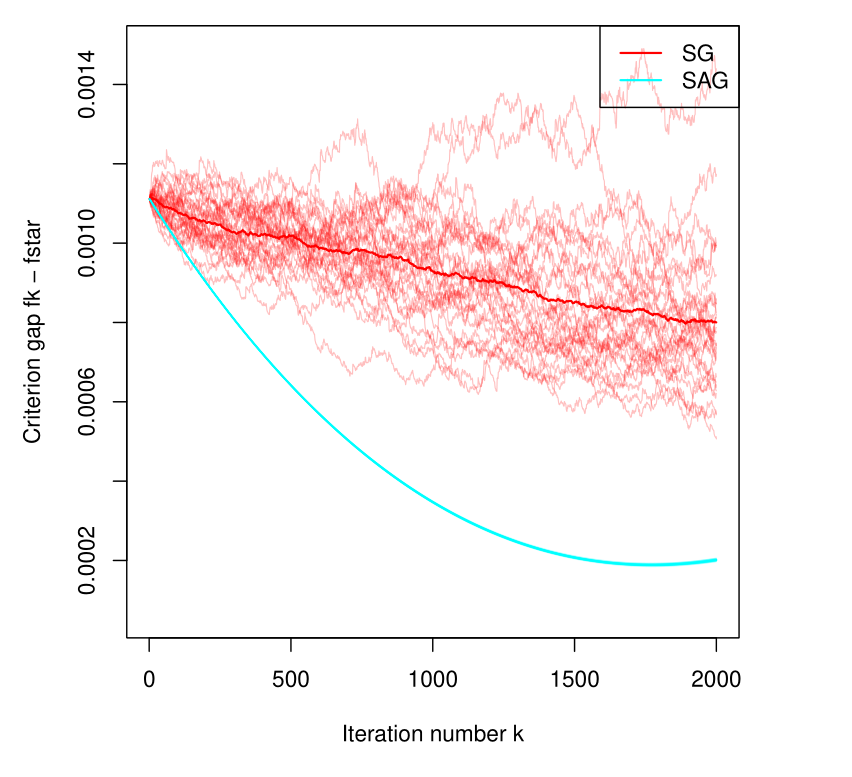
\includegraphics[width=\textwidth,height=\textheight,keepaspectratio]{SAG.png}
    \caption{\label{fig:label} }
  \end{figure}

\end{frame}


\section{SAGA}%
\label{sec:}

\begin{frame}
  \frametitle{SAGA, 2014}
  Very similar:
  \begin{itemize}
    \item maintain table containing gradients $g_i$ of $f_i$
    \item at step $k = 1,2, \dots$ pick random $i_k \in [n]$ and
          \begin{equation}
            g_i^k := \nabla f_{i_k}(x^{k})
          \end{equation}
          set $g_{i}^k = g_i^{k-1}$ for all $i\neq i_k$ (remain the same)
    \item Update
          \begin{equation}
            x^{k+1} = x^k -u \alpha_k  \Big( g_{i_k}^k - g_{i_k}^{k-1} + \frac{1}{n}\sum_{i=1}^{n} g_i^k \Big)
          \end{equation}
    \item estimator now \textbf{unbiased}!
  \end{itemize}
\end{frame}

\begin{frame}
  \frametitle{For Comparison}
  SAGA gradient estimate:
  \begin{equation}
    g_{i_k}^k - g_{i_k}^{k-1} + \frac{1}{n}\sum_{i=1}^{n} g_i^k
  \end{equation}

  SAGA gradient estimate:
  \begin{equation}
    \frac{1}{n}g_{i_k}^k - \frac{1}{n}g_{i_k}^{k-1} + \frac{1}{n}\sum_{i=1}^{n} g_i^k
  \end{equation}

\end{frame}

\begin{frame}
  \frametitle{}

  \begin{figure}[ht]
    \centering
    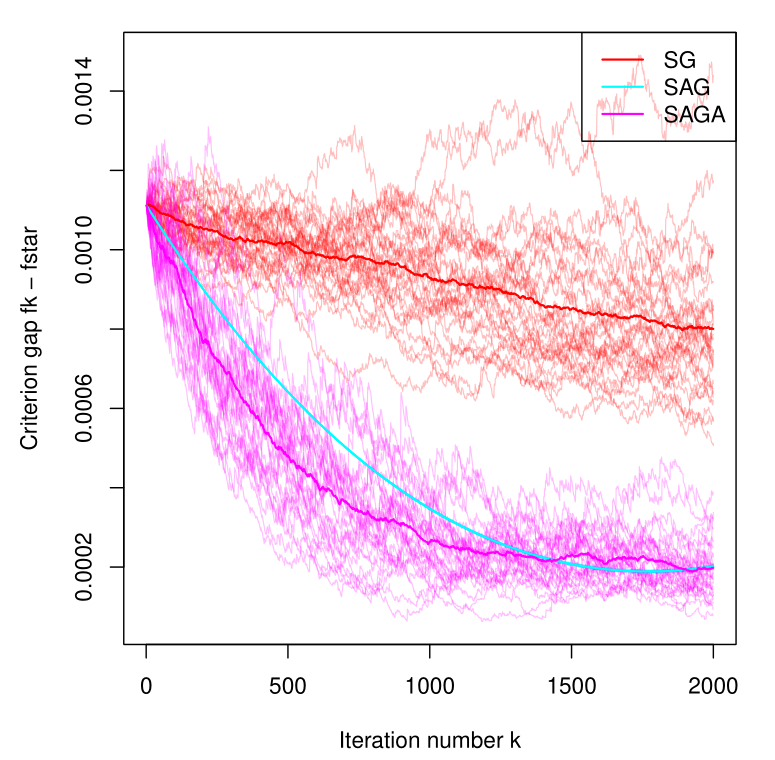
\includegraphics[width=\textwidth,height=\textheight,keepaspectratio]{SAGA.png}
    % \caption{\label{fig:label} }
  \end{figure}
  Highlights the low variance of SAG.
\end{frame}


\section{SVRG}%

\begin{frame}
  \frametitle{Stochastic Variance Reduced Gradient (SVRG), 2013}

  \begin{algorithm}[H]
    \caption{SVRG}\label{}
    \begin{algorithmic}[1]
      \For{$k=1,2, \dots$}
      \State{Set $x^1 = \tilde{x} = \tilde{x}^{k}$}
      \State{Compute $\tilde{\mu} := \nabla f(\tilde{x})$ \hfill \textcolor{blue}{//update snapshot}}
      \For{$l=1,2, \dots, m$ }\hfill \textcolor{blue}{//$m$ iterations per epoch}
      \State{pick $i_l$ uniform at random in $[n]$}
      \State{Set $x^{l+1} = x^l - \alpha (\nabla f_{i_l}(x^l) - \nabla f_{i_l}(\tilde{x}) + \tilde{\mu})$}
      \EndFor{}
      \State{$\tilde{x}^{k+1}= x^{m+1}$}
      \EndFor{}
    \end{algorithmic}
  \end{algorithm}

  \begin{itemize}
    \item Does \textbf{not} need to \textbf{store} full table of gradients.
    \item requires \emph{batch} gradient computation every \emph{epoch}
    \item per iteration cost is comparable to that of SGD if $m \ge n$
    \item convergence rates similar to SAGA, but simpler analysis.
  \end{itemize}
\end{frame}

\begin{frame}
  \frametitle{SVRG}
  \textbf{key idea:} by storing old point we can
  \begin{equation}
    \underbrace{\nabla f_{i_k}(x^k) - \nabla f_{i_k}(x^{\text{old}})}_{\text{$\to 0$ if $x\approx x^{\text{old}}$}} + \underbrace{\nabla f(x^{\text{old}})}_{\text{$\to 0$ if $x^{\text{old}}$}}
  \end{equation}
  \begin{itemize}
    \item is an unbiased estimate of $\nabla f(x^k)$
    \item converges to $0$ (meaning reduced variability) if $x^k\approx x^{\text{old}} \approx x^*$
  \end{itemize}

\end{frame}

% talk about \sqrt{n} improvement
% talk about loopless svrg?


\end{document}
